%% Example data sheet
%% Feel free to modify and use this file for any purpose, under
%% either the LaTeX Project Public License or under public domain.

% Options here are passed to the article class.
% Most common options: 10pt, 11pt, 12pt
\documentclass[10pt]{datasheet}

% Input encoding and typographical rules for English language
\usepackage[utf8]{inputenc}
\usepackage[english]{babel}
\usepackage[english]{isodate}

% tikz is used to draw images in this example, but you can
% also use \includegraphics{}.
\usepackage{tikz}
\usepackage{pgfplots}
\usepackage{circuitikz}
\usetikzlibrary{calc}

% These define global texts that are used in headers and titles.
\title{Example Data Sheet}
\author{Fancy Company}
\date{November 2020}
\revision{Revision 1}
\companylogo{\Huge $\nabla$ Fancy Company}

\begin{document}
\maketitle

\section{Features}

\begin{itemize}
\item{Classic datasheet style in LaTeX}
\item{Write math equations as easy as $e^{i \pi}$}
\item{Easy to use document class}
\end{itemize}

\section{Applications}

\begin{itemize}
\item{Data sheets for electronics components}
\item{Technical sales brochures}
\item{Functional specifications}
\end{itemize}

\section{General Description}
The \textbf{datasheet} document class makes it easy to write great looking
data sheets using the LaTeX typesetting system. It follows the classic style used
by most manufacturers of electronic components.

You can download the document class from
\href{https://github.com/PetteriAimonen/latex-datasheet-template/}{latex-datasheet-template}
GitHub repository.
The repository includes this example datasheet as \textbf{example.tex} and
the document class as \textbf{datasheet.cls}.
You can build the PDF document using command \texttt{latexmk -pdf}.

% Switch to next column
\vfill\break

\begin{figure}[h]
    \begin{circuitikz}[european]
        \node[op amp] (amp1) {};
        \node[op amp, below = 0.5cm, xscale = -1] (amp2) {};
        \draw (amp1.out) |- (amp2.-);
        \draw (amp2.-) ++(0, 0.3cm) node[circ]{} to +(2,0) node[above left]{5};
        \draw (amp2.out) to (amp1.+);
        \draw (amp1.+) ++(0, -0.3cm) node[circ]{} to +(-2,0) node[above right]{2};
        \draw (amp1.-) to +(-2,0) node[above right]{1};
        \draw (amp2.+) to +(2,0) node[above left]{4};
        \draw (amp1.out) +(0,0.5cm) node (Vdd) {$\mathrm{V_{DD}}$};
        \draw (Vdd.east) to +(1.5,0) node [above left]{6};
        \draw (amp2.out) +(0,-0.5cm) node (Vss) {$\mathrm{V_{SS}}$};
        \draw (Vss.west) to +(-1.6,0) node [above right]{3};
        \draw ($(amp1.north west) + (-0.5,0.5)$) rectangle ($(amp2.south west) + (0.5,-0.5)$);
    \end{circuitikz}
    \caption{Pinout and internal circuit}
\end{figure}

\begin{figure}[h]
    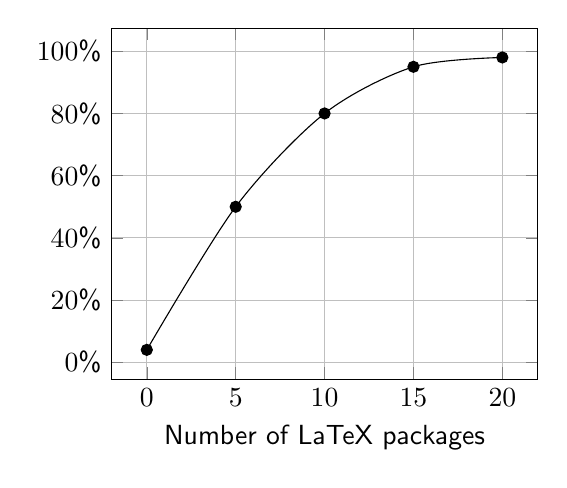
\begin{tikzpicture}
        \sffamily
        \begin{axis}[
            width=7cm,
            xlabel={Number of LaTeX packages},
            ytick distance=20,
            yticklabel={\pgfmathprintnumber{\tick}\%},
            xmajorgrids, ymajorgrids]
        \addplot[smooth,mark=*] plot coordinates {
            (0,4)
            (5,50)
            (10,80)
            (15,95)
            (20,98)
        };
        \end{axis}
    \end{tikzpicture}
    \caption{Typical data sheet production efficiency}
\end{figure}

% For wide tables, a single column layout is better. It can be switched
% page-by-page.
\onecolumn

\section{Electrical Specifications}
All specifications are in $-40\degree C \leq T_A \leq 85\degree C$ unless otherwise noted.

\begin{table}[h]
\begin{threeparttable}
\caption{Example Data Sheet Specifications}
\begin{tabularx}{\textwidth}{l | c | c c c | c | X}
    \thickhline
    \textbf{Parameter} & \textbf{Symbol} & \textbf{Min.} & \textbf{Typ.} & \textbf{Max.} &
    \textbf{Unit} & \textbf{Conditions} \\
    \hline
    Page width  & $p_w$ & 20.9 & 21.0 & 21.1 & cm & \multirow{2}{*}{Standard A4 paper} \\
    Page height & $p_h$ & 29.6 & 29.7 & 29.8 & cm &  \\
    \hline
    Insulation voltage & $E_{max}$\tnote{1} & & 1 & & kV & \\
    \thickhline
\end{tabularx}
\begin{tablenotes}
\item[1]{Based on characterization data, not tested in production.}
\end{tablenotes}
\end{threeparttable}
\end{table}

\section{Absolute Maximum Ratings}

\begin{table}[h]
\caption{Absolute Maximum Ratings of Example Data Sheet}
\begin{tabularx}{\textwidth}{l | X}
    \thickhline
    \textbf{Parameter} & \textbf{Rating} \hspace{5cm} \\
    \hline
    Daily exposure to LaTeX & 24 hours \\
    \thickhline
\end{tabularx}
\end{table}

\textbf{Note:} Stresses above those listed under Absolute Maximum Ratings can
cause permanent damage to the device. This is a stress rating only. Functional
operation of the device is not implied in any conditions above those indicated
in the Electrical Specifications section.

\end{document}

